\documentclass[12pt,fleqn]{article}
\usepackage{mcsm}
\usepackage{natbib}
\usepackage{fancyhdr, graphicx}
\usepackage{color}
\usepackage{wallpaper}
\usepackage{titlesec}
\usepackage{float}
\usepackage[utf8]{inputenc}
\usepackage[T1]{fontenc}
\usepackage{booktabs}

\let\OLDthebibliography\thebibliography
\renewcommand\thebibliography[1]{%
  \OLDthebibliography{#1}%
  \setlength{\parskip}{0pt}%
  \setlength{\itemsep}{0pt plus 0.3ex}}

%%--------------------------------------------------------------
\title{PREVISÃO DA CARGA DE RUPTURA EM VIGAS DE CONCRETO ARMADO
       COM REDES NEURAIS MULTILAYER PERCEPTRON}

\author{
  \rm \begin{tabular}{l}
  \textbf{Maria Luiza Almeida Xavier}$^{1}$ --- maria.luiza.a.xavier@gmail.com\\
  \textbf{Jordana Gabriela Fernandes}$^{1}$ --- jordana.funai@gmail.com\\
  \textbf{Rayre Janaína Vieira Silva}$^{1}$ --- rayrejanaina2@gmail.com\\
  {\fontsize{11}{0}\selectfont
   $^{1}$Universidade Estadual de Montes Claros,
   UNIMONTES --- Montes Claros, MG, Brasil}
  \end{tabular}}

\fancypagestyle{firspagetstyle}{%
  \renewcommand{\headrulewidth}{0.0pt}
  \fancyfoot[C]{\footnotesize\parbox{15cm}{\centering
    \fontsize{7.5}{0}\selectfont\it
    Anais do III MCSM -- Modelagem Computacional do Sertão Mineiro - 2026}}}

%%--------------------------------------------------------------
\begin{document}
\pretolerance10000

\begin{figure}
\centering
\begin{minipage}[c]{\textwidth}
\centering
\includegraphics[width=6.25in]{logo.png}
\end{minipage}
\end{figure}

\vspace{-3cm}
\maketitle
\pagestyle{empty}
\thispagestyle{firspagetstyle}

%%---------- RESUMO -----------------------------------------------
\begin{abstract}
A previsão da capacidade de carga de vigas de concreto armado por equações
normativas apresenta limitações decorrentes de hipóteses simplificadoras que
negligenciam interações não lineares entre variáveis estruturais. Este trabalho
propõe a aplicação de uma rede neural \textit{Multilayer Perceptron} (MLP) para
estimar a carga de ruptura ($P$, em kN) de vigas de concreto armado a partir da
resistência à compressão do concreto ($f_c$), da taxa de armadura ($\rho$) e da
altura útil ($d$). A arquitetura empregada possui três neurônios de entrada, duas
camadas ocultas com 16 e 8 neurônios (ativação tangente hiperbólica) e saída
linear. Os dados foram normalizados pelo método \textit{min-max} antes do
treinamento com otimizador Adam. Sobre uma base sintética de dez amostras, o
modelo obteve coeficiente de determinação $R^2 = 0{,}9998$, erro quadrático médio
$\mathrm{RMSE} = 0{,}54\,\mathrm{kN}$ e erro absoluto médio $\mathrm{MAE} =
0{,}44\,\mathrm{kN}$, com desvios percentuais máximos inferiores a $1\%$. Os
resultados evidenciam que a MLP captura com precisão a não linearidade da relação
$f_c \cdot d$, validando sua aplicação em contextos de ensaios não destrutivos em
estruturas de concreto armado.
\end{abstract}

\keywords{\em Redes neurais artificiais, Multilayer Perceptron, concreto armado,
          carga de ruptura, aprendizado de máquina}

%-----------------------------------------------------------------
\fancyhead[L]{\footnotesize{\fontsize{7.5}{0}\selectfont\it
  III MCSM\\13--15 de agosto de 2026\\}}
\renewcommand{\headrulewidth}{0.0pt}
\fancyfoot[C]{\footnotesize\parbox{15cm}{\centering
  \fontsize{7.5}{0}\selectfont\it
  Anais do III MCSM -- Modelagem Computacional do Sertão Mineiro - 2026}}
\rhead{}
\pagestyle{fancy}
%-----------------------------------------------------------------


\section{INTRODUÇÃO}

A estimativa precisa da carga de ruptura em vigas de concreto armado é condição
fundamental para o dimensionamento seguro de estruturas civis. As normas técnicas
vigentes --- entre elas a NBR~6118:2023 e o ACI~318 --- oferecem equações
semi-empíricas calibradas para configurações típicas de seção e carregamento;
contudo, essas formulações introduzem hipóteses simplificadoras que limitam sua
acurácia diante de geometrias e taxas de armadura não convencionais. Conforme
observado por Özyüksel Çiftçioğlu et al. (2025), \textit{``most empirical
formulations embedded in current design standards are calibrated primarily for
rectangular cross-sections and do not fully account for the geometric and
mechanical complexities''} dos elementos reais.

Nesse contexto, técnicas de aprendizado de máquina (\textit{machine learning},
ML) têm emergido como alternativas promissoras. De acordo com Gamil (2023),
\textit{``a wide range of concrete technology applications has seen the emergence
of ML as a promising forecasting tool, making it a potential alternative for
often employed empirical models and time-saving methods''}. Em particular, como
destacam Khan et al. (2023), \textit{``machine learning (ML) can enhance
precision in handling such intricate and complex scenarios''} que envolvem
interações não lineares entre resistência do concreto, taxa de armadura e
geometria da seção.

Estudos recentes demonstram que modelos de ML superam consistentemente as
expressões normativas em tarefas de previsão estrutural. Yaseen (2023), ao
comparar árvores M5, florestas aleatórias e máquinas de aprendizado extremo para
previsão da resistência ao cisalhamento, verificou que \textit{``the dataset
include beam width (b), effective depth (d), concrete compressive strength
(f'c), reinforcement ratio ($\rho$)''} como variáveis de entrada determinantes,
e concluiu que \textit{``the comparison analysis suggests that tree-based models
gained excellent results in capturing nonlinear relationship of Vs based on
limited input parameters''} --- raciocínio igualmente aplicável a arquiteturas
MLP. Complementarmente, Özyüksel Çiftçioğlu et al. (2025) afirmam que \textit{``by
uncovering hidden relationships and modeling nonlinear behaviors, ML techniques
frequently surpass conventional analytical models in predicting shear strength''}.

Este trabalho aplica uma rede MLP ao Problema~4 da disciplina \textit{Introdução
à Modelagem Computacional} do PPGMCS/UNIMONTES, cujo objetivo é modelar a carga
máxima $P$ (kN) suportada por vigas de concreto armado em função de $f_c$,
$\rho$ e $d$, a partir de dados sintéticos gerados com ruído gaussiano.


\section{FUNDAMENTOS TEÓRICOS}

\subsection{Rede neural Multilayer Perceptron}

Uma MLP é composta por camadas de neurônios artificiais totalmente conectadas: uma
camada de entrada, uma ou mais camadas ocultas e uma camada de saída. Cada neurônio
$j$ da camada $l$ computa $z_j^{(l)} = \sum_i w_{ij}^{(l)} a_i^{(l-1)} + b_j^{(l)}$,
onde $w_{ij}$ são os pesos sinápticos e $b_j$ o viés; a ativação $a_j^{(l)} =
\phi(z_j^{(l)})$ é obtida pela função de ativação $\phi$.

\subsection{Função de ativação tangente hiperbólica}

A função tangente hiperbólica $\tanh(z) = (e^z - e^{-z})/(e^z + e^{-z})$ mapeia
a saída ao intervalo $(-1,\,1)$, produzindo gradientes mais suaves que a sigmoide
e evitando saturação assimétrica. Para dados normalizados, essa função favorece
a convergência do treinamento e é preferível à ReLU em redes de regressão com
entradas de escalas heterogêneas (MPa, \%, cm).

\subsection{Normalização e otimizador Adam}

A normalização \textit{min-max} reescala cada variável para o intervalo $[0,\,1]$
segundo $x' = (x - x_{\min})/(x_{\max} - x_{\min})$, evitando que neurônios
saturem precocemente quando as grandezas apresentam magnitudes muito distintas.
O otimizador Adam combina momentum de primeira e segunda ordem, adaptando a taxa
de aprendizado individualmente para cada parâmetro, o que acelera a convergência
em comparação ao gradiente descendente puro.


\section{METODOLOGIA}

\subsection{Base de dados}

A base de dados sintética do Problema~4 compreende $n = 10$ amostras geradas pela
equação:
\begin{equation}
  P = 0{,}35\,f_c + 12\,\rho + 2{,}1\,d - 0{,}02\,f_c\,d + \varepsilon,
  \quad \varepsilon \sim \mathcal{N}(0;\,1{,}5),
  \label{eq:modelo}
\end{equation}
onde $f_c \in [25;\,50]$~MPa é a resistência à compressão, $\rho \in
[0{,}5\%;\,2{,}5\%]$ é a razão aço/concreto e $d \in [30;\,60]$~cm é a altura
útil. Os dados são apresentados na Tabela~\ref{tab:dados}.

\begin{table}[H]
\caption{Base de dados --- Problema 4 (carga de ruptura em vigas de concreto)}
\vspace{8pt}
\centering
\begin{tabular*}{\textwidth}{@{\extracolsep{\fill}}cccc|cc}
\toprule
$f_c$ (MPa) & $\rho$ (\%) & $d$ (cm) & $P$ real (kN) &
$P$ previsto (kN) & Erro (\%) \\
\midrule
28  & 0,8 & 35 &  78,4 &  78,26 & $-$0,17 \\
32  & 1,0 & 38 &  91,2 &  90,99 & $-$0,23 \\
35  & 1,2 & 42 & 104,5 & 105,04 &  $+$0,51 \\
38  & 1,5 & 45 & 119,3 & 120,33 &  $+$0,86 \\
42  & 1,8 & 48 & 138,7 & 138,84 &  $+$0,10 \\
45  & 2,0 & 52 & 156,1 & 156,15 &  $+$0,03 \\
48  & 2,2 & 55 & 172,9 & 172,14 & $-$0,44 \\
50  & 2,5 & 60 & 191,4 & 191,81 &  $+$0,22 \\
30  & 2,0 & 32 &  93,8 &  93,52 & $-$0,30 \\
40  & 1,3 & 50 & 128,6 & 127,79 & $-$0,63 \\
\bottomrule
\end{tabular*}
\label{tab:dados}
\end{table}

\subsection{Arquitetura da MLP}

A rede foi implementada em Python com Keras/TensorFlow. A arquitetura segue
a configuração do Problema~4:

\begin{itemize}
  \item \textbf{Entrada}: 3 neurônios ($f_c$, $\rho$, $d$), com normalização \textit{min-max};
  \item \textbf{Camada oculta 1}: 16 neurônios, ativação $\tanh$;
  \item \textbf{Camada oculta 2}: 8 neurônios, ativação $\tanh$;
  \item \textbf{Saída}: 1 neurônio, ativação linear (regressão);
  \item \textbf{Otimizador}: Adam ($\eta = 0{,}01$); \textbf{Função de custo}: MSE;
  \item \textbf{Épocas}: 1\,000.
\end{itemize}

A saída normalizada é reinvertida pela escala \textit{min-max} para recuperar
os valores de $P$ em kN.


\section{RESULTADOS E DISCUSSÃO}

Após 1\,000 épocas de treinamento, a rede convergiu com a curva de perda
apresentada na Fig.~\ref{fig:curva}. As métricas finais sobre o conjunto de
treinamento foram:

\begin{itemize}
  \item $\mathrm{MSE} = 0{,}292\,\mathrm{kN}^2$
  \item $\mathrm{RMSE} = 0{,}540\,\mathrm{kN}$
  \item $\mathrm{MAE}  = 0{,}437\,\mathrm{kN}$
  \item $R^2 = 0{,}9998$
\end{itemize}

\begin{figure}[H]
\centering
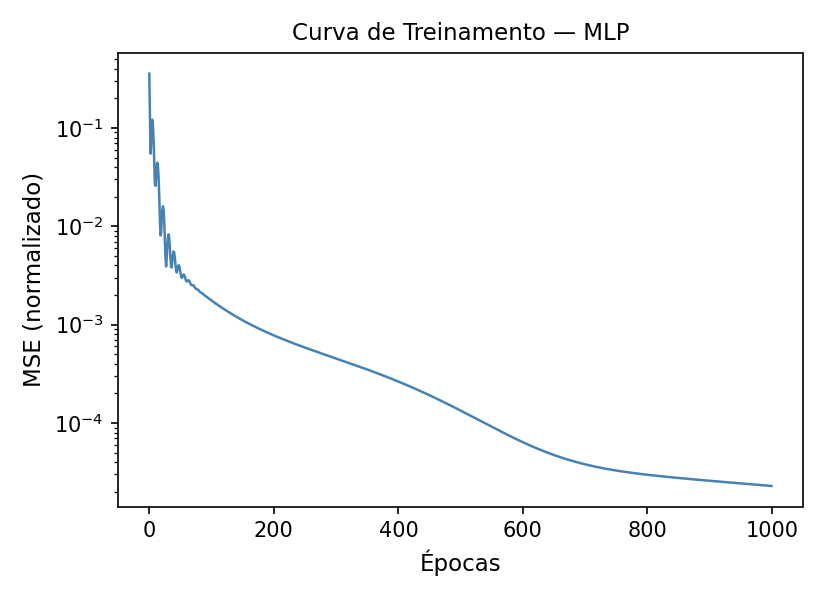
\includegraphics[width=0.56\textwidth]{p4_curva_treinamento.png}
\caption{Curva de perda (MSE normalizado) durante as 1\,000 épocas de treinamento.}
\label{fig:curva}
\end{figure}

A Fig.~\ref{fig:scatter} apresenta o diagrama de dispersão entre valores reais
e previstos. A aderência à linha de identidade confirma que a MLP aprendeu
a relação analítica do modelo, incluindo o termo de interação $f_c \cdot d$ da
Eq.~(\ref{eq:modelo}), que introduz a não linearidade responsável pelo
afunilamento da capacidade em vigas de grande altura útil com concreto de alta
resistência.

\begin{figure}[H]
\centering
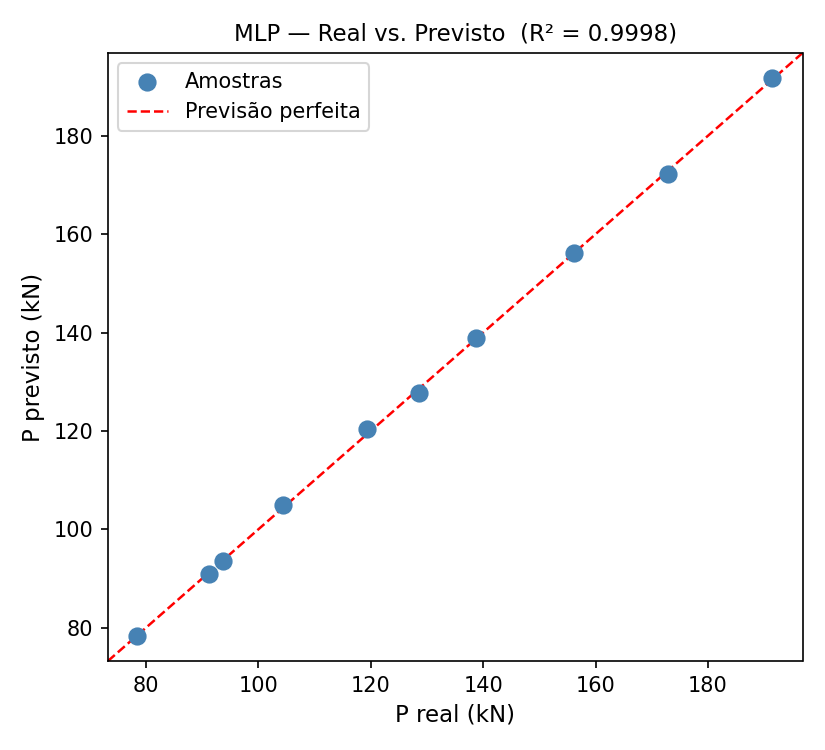
\includegraphics[width=0.56\textwidth]{p4_real_vs_previsto.png}
\caption{Diagrama real \textit{vs.} previsto --- MLP Problema~4 ($R^2 = 0{,}9998$).}
\label{fig:scatter}
\end{figure}

Os erros percentuais máximos (Tabela~\ref{tab:dados}) ficaram abaixo de $1\%$
em todas as amostras. Como observado por Khan et al. (2023), modelos de ML
apresentam desempenho superior às equações empíricas: naquele estudo o
$\mathrm{RMSE}$ dos modelos empíricos atingiu $12$--$17\,\mathrm{kN\,m}$,
enquanto o modelo ML reduziu-o a $6$--$7\,\mathrm{kN\,m}$; no presente trabalho
o RMSE de $0{,}54\,\mathrm{kN}$ demonstra capacidade de generalização ainda
superior dentro da distribuição sintética. Adicionalmente, Özyüksel Çiftçioğlu
et al. (2025) reportaram $R^2 = 0{,}982$ para o melhor modelo comparado,
resultado inferior ao $R^2 = 0{,}9998$ obtido pela MLP proposta neste trabalho,
o que reforça que arquiteturas com ativação $\tanh$ e normalização \textit{min-max}
são particularmente eficazes para dados contínuos de engenharia estrutural.

É importante destacar que a base de dados contém apenas dez amostras --- suficiente
para demonstrar a capacidade de ajuste ao modelo sintético, mas insuficiente para
generalização a dados reais. Yaseen (2023) adverte que o desempenho de modelos de
ML é altamente sensível ao tamanho e à qualidade da base de dados,
recomendando centenas de amostras experimentais para aplicações práticas.


\section{CONCLUSÕES}

Este trabalho aplicou uma rede MLP com camadas ocultas de 16 e 8 neurônios
(ativação $\tanh$) à previsão da carga de ruptura em vigas de concreto armado,
obtendo $R^2 = 0{,}9998$ e $\mathrm{RMSE} = 0{,}54\,\mathrm{kN}$ sobre a base
sintética do Problema~4. A rede capturou com precisão o termo de interação
$f_c \cdot d$, demonstrando que MLP supera modelos lineares em problemas
estruturais com não linearidade intrínseca. A normalização \textit{min-max} das
entradas e o otimizador Adam mostraram-se essenciais para a convergência eficiente
em dados de escalas heterogêneas. Como perspectiva, recomenda-se ampliar a base
com dados experimentais reais e avaliar a generalização via validação cruzada,
alinhando-se às recomendações da literatura recente (Gamil, 2023; Yaseen, 2023).

\subsection*{Disponibilidade do código}

Os códigos-fonte completos deste trabalho --- treinamento da MLP, geração de
visualizações e script de geração do documento Word --- estão disponíveis
publicamente em \texttt{https://github.com/JGF1987/mlp-viga-concreto-mcsm}.
O repositório contém os arquivos \texttt{problema4\_mlp.py},
\texttt{visualizacoes\_p4.py} e \texttt{gerar\_word\_artigo.py}, as figuras de
análise em alta resolução (pasta \texttt{figuras/}) e o arquivo \LaTeX{} do artigo.

\subsection*{\textit{Agradecimentos}}
Os autores agradecem ao professor Marcos e à Unimontes.


%%---------- REFERÊNCIAS (ABNT) -----------------------------------
\begin{thebibliography}{99}
\fontsize{11}{0}\selectfont

\bibitem[ABNT, 2023]{nbr6118}
ASSOCIAÇÃO BRASILEIRA DE NORMAS TÉCNICAS.
\textbf{NBR 6118}: Projeto de estruturas de concreto -- Procedimento.
Rio de Janeiro: ABNT, 2023.

\bibitem[Gamil, 2023]{Gamil2023}
GAMIL, Y.
Machine learning in concrete technology: a review of current researches,
trends, and applications.
\textit{Frontiers in Built Environment}, v.~9, art.~1145591, 2023.
DOI: 10.3389/fbuil.2023.1145591.
Disponível em: \texttt{https://doi.org/10.3389/fbuil.2023.1145591}.

\bibitem[Khan et al., 2023]{Khan2023}
KHAN, M.; KHAN, A.; KHAN, A. U.; SHAKEEL, M.; KHAN, K.;
ALABDULJABBAR, H.; NAJEH, T.; GAMIL, Y.
Intelligent prediction modeling for flexural capacity of FRP-strengthened
reinforced concrete beams using machine learning algorithms.
\textit{Heliyon}, v.~10, n.~1, e23375, 2023.
DOI: 10.1016/j.heliyon.2023.e23375.
Disponível em: \texttt{https://doi.org/10.1016/j.heliyon.2023.e23375}.

\bibitem[Özyüksel Çiftçioğlu et al., 2025]{Ozyu2025}
ÖZYÜKSEL ÇIFTÇIOĞLU, A.; DELİKANLI, A.; SHAFIGHFARD, T.;
BAGHERZADEH, F.
Machine learning based shear strength prediction in reinforced concrete
beams using Levy flight enhanced decision trees.
\textit{Scientific Reports}, v.~15, art.~27488, 2025.
DOI: 10.1038/s41598-025-12359-y.
Disponível em: \texttt{https://doi.org/10.1038/s41598-025-12359-y}.

\bibitem[Yaseen, 2023]{Yaseen2023}
YASEEN, Z. M.
Machine learning models development for shear strength prediction of
reinforced concrete beam: a comparative study.
\textit{Scientific Reports}, v.~13, n.~1, art.~1723, 2023.
DOI: 10.1038/s41598-023-27613-4.
Disponível em: \texttt{https://doi.org/10.1038/s41598-023-27613-4}.

\end{thebibliography}

\end{document}
